\section{Theoretical Approach}
Experimental coincidence spectra are given by the kinetic energies $E_{sec}$
of the secondary electron
and the intensities of the peaks. The latter is proportional to the
probability of the decay as well as the theoretically determinable
decay width $\Gamma=\frac{\hbar}{\tau}$,
which is inverse proportional to the lifetime $\tau$. The manifold of the
secondary energies and decay widths will therefore compose the electron-electron
coincidence spectrum.
In case of noble gas clusters
with given structures three aspects have to be taken into account:
different decay mechanisms, the possibility to decay with multiple
interaction partners and different decay channels within each decay mechanism.
At the current stage of development we need to neglect the nuclear dynamics which
additionally might play an important role.

This means we are dealing with a sum over three different indices for the
evaluation of the decay width. For a given structure it is most convenient to
start with a decomposition of the total system into interaction partners of
the different decay mechanisms, i.e. pairs (combination of two atoms regardless
the internuclear distance) for the ICD and triples (combinations of three atoms)
for the ETMD.
These atoms do not necessarily need to form bonds between each other or
even be close, but they are characterized according to fixed internal
coordinates. Each pair and triple can be described by its properties, like
energy of the secondary electron and decay width,
which are in first order of approximation independent of further, eventually
present, atoms. In the following, this approach is going to be called
model of pairs and triples.


%Decomposing every system into pairs and triples of atoms is a very useful
%first order approximation to both the investigation of energies and
%decay widths of a larger system. Pairs and triples are combinations of
%two and three atoms, respectively.

In order to determine, whether a channel $\beta$ for a given geometry and decay
mechanism is open ,i.e., in accordance with energy conservation,
the energies of the initial $E_{in}$ and the final states $E_{fin}$ of
the corresponding processes are necessary.
When the channel
is open, the excess energy is carried away by the emitted electron $E_{sec}$
in form of its kinetic energy. These energies can in the model
of pairs and triples be approximated to be

\begin{align}
 E_{in}        &= SIP(X_{in}) \label{equation:E_in}\\
 E_{fin}^\beta &= SIP(X_{D}^\beta) + SIP(X_{E}^\beta) + \frac 1d
           \label{equation:E_fin}\\
 E_{sec}^\beta &= E_{in}^\beta - E_{fin}^\beta \label{equation:E_sec}
\end{align}
where $X_{in}$ denotes the initially ionized atom and
$X_{D}$ and $X_{E}$ describe the electron donating atom and electron
emitting atom, respectively.
$\beta$ denotes the decay channel characterized
by the quantum numbers of the ionized atoms in the pairs
and triples and $d$ denotes the interatomic distance between the atoms
$X_{D}$ and $X_{E}$. The initially ionized atom $X_{in}$ can
coincide with one or both of
the final state atoms
$X_{D}$ and $X_{E}$.
The distribution of the vacancies over the different
atoms determines the kind of electronic decay process at hand. Hence, in an
Auger process all three atoms would coincide, for an ICD $X_{in}$
would coincide with $X_{D}$ and for an {ETMD}3
all ionized states are located on different atoms.

\begin{figure}[h]
 \centering
 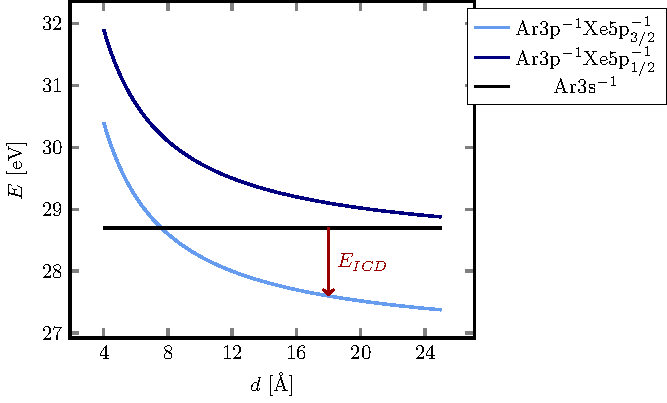
\includegraphics[width=8.5cm]{pics/channel_open_ICD.pdf}
 \caption{Initial and final state energies for ArXe pairs at different
          distances using the experimental ionization potentials as given
          in Table \ref{}. For distances larger than the channel opening
          distance the ICD channel is open.}
 \label{figure:channel_open_ICD}
\end{figure}

In all autoionization processes considered, a second electron
is emitted with the kinetic energy $E_{sec}$. If $E_{sec}<0$, then
the final state energy is higher than the initial state energy and the        
process is energetically not accessible. Hence, the corresponding channel     
is closed as shown in Figure \ref{figure:channel_open_ICD}. Related to
the opening of each channel is an internuclear distance which we in the
following call \emph{channel opening distance}.
                                                               
This ad hoc approach easily allows to correct for energetic shifts of         
ionization potentials as observed in larger clusters by adding experimentally
or theoretically determined energy shifts $\Delta E(X_{A}^{\beta})$
for a given role in the decay
$A=in,D,E$ and a channel $\beta$ which yields
the working expression for the kinetic energy of the secondary electron

\begin{equation}
 E_{sec}^\beta = SIP(X_{in}) + \Delta E (X_{in})
               - SIP(X_{D}^\beta) - \Delta E (X_{D}^\beta)
               - SIP(X_{E}^\beta) - \Delta E (X_{E}^\beta)
               - \frac 1d .
\end{equation}

The total decay width $\Gamma$ is given by the sum over the decay widths
of all decay mechanisms. In case of the ArXe clusters we only consider
ICD and ETMD:

\begin{equation}
 \Gamma = \Gamma_{ICD} + \Gamma_{ETMD} .
\end{equation}

These are given by the sum over the decay widths of all pairs $i$ for the
ICD and all triples $j$ for the ETMD3, respectively and all channels $\beta$.

\begin{align}
 \Gamma_{ICD}  &= \sum\limits_{i,\beta} N_{ICD,i}  \, \Gamma_{ICD,i,\beta}\\
 \Gamma_{ETMD} &= \sum\limits_{j,\beta} N_{ETMD,j} \, \Gamma_{ETMD,j,\beta}\\
\end{align}
Here, $N_{ICD,i}$ and $N_{ETMD,j}$ denote the number of geometrically
equal pairs and triples in a given cluster structure. The total number of pairs
reads
$N_{ICD} = N_{in} \cdot N_{D/E} = N_{Ar} \cdot N_{Xe}
 = \sum\limits_i N_{ICD,i}$ and the number of triples as
$N_{ETMD} = N_{in} \cdot N_{D/E} (N_{D/E} - 1) = N_{Ar} \cdot N_{Xe} (N_{Xe} - 1)
 = \sum\limits_j N_{ETMD,j}$.
The number of geometrically equal pairs $N_{ICD,i}$ and $N_{ETMD,j}$
strongly depend on the structure of the cluster. From these relationships
it can be seen that a higher xenon content in the cluster statistically
favours the ETMD3 over the ICD.

In previous work \cite{Fasshauer13,Fasshauer_PhD} we have shown that
the decay width for a single pair or triple for a distinct channel $\beta$
following Wentzel \cite{Wentzel27}, Feshbach\cite{Feshbach58,Feshbach62}
and Fano \cite{Fano61}

\begin{equation}
 \Gamma_{\beta}(E_{res}) = 2\pi \left|
                           \braket{\Phi_{in}| H_f |\chi_{\beta}}
                           \right|^2
\end{equation}

can be approximated by its asymptotic behaviour

\begin{equation}
 \Gamma_{ICD,i,\beta} = 2\pi
                        \frac{\sigma^{(X_E)}(\omega_{vp,\beta})}
                        {R_i^6 \, \omega_{vp,\beta}^4 \tau_{in,\beta}}
\end{equation}


\begin{equation}
 \Gamma_{ETMD,j,\beta} = 2\pi \sum\limits_{m,M_{in}',D}
                        \frac{a_m \Theta_m(\alpha_j) \sigma^{(X_E)}(\omega_{vp,\beta})
                              \tilde{D}_{m,j,\beta}(M_{in,D},M_{in,D'})}
                         {R_j^6 \omega_{vp,\beta}}
\end{equation}

depending on constants ($a_m=4,2$) as well as experimental properties
of atoms like ionization cross sections
$\sigma^{(X_E)}(\omega_{vp,\beta})$, radiative lifetimes of the initially
ionized state $\tau_{in,\beta}$ and the excess energy transferred to the
emitting atom (the energy of the virtual photon) $\omega_{vp,\beta}$
and calculated dipole transition moments $\tilde{D}_{m,j,\beta}$, only.
Here, $\Theta_m(\alpha_j)$ is a function depending on the angle $\alpha_j$
of the triple (compare Ref. \cite{Fasshauer13}).

In this work we evaluate the secondary energies and decay widths with
the program HARDRoC \cite{} using the
experimental ionization energies of Table \ref{}
and data from the literature given in Tables \ref{} and \ref{}.
These are the same as the ones used in Reference \cite{Fasshauer13}.
